\section{Implementation}
Um die Feldlinien darzustellen müssen diese heruntergeladen und dekomprimiert werden. Die zwei Operationen sind die Hauptverantwortlichen für die Wartezeit. Um die Wartezeit zu verkürzen, werden Feldlinien bereits im Voraus asynchron heruntergeladen. Somit sind die Daten bereits im Arbeitsspeicher, bevor die Visualisierung sie benötigt.\\
Die Wartezeit kann mit zusätzlichen Massnahmen weiter verkürzt werden Folgende Massnahmen wurden implementiert:
\begin{enumerate}
	\item Asynchrone Dekompression.
	\item Vorladen der Dekomprimierten Feldlinien.
	\item Mehrstufiges Caching.
\end{enumerate}
Während der Benutzer sich eine Aufnahme der Feldlinie sieht, soll asynchron bereits die nächsten Aufnahmen heruntergeladen und dekomprimiert werden. So ist der Wechsel von Aufnahme zu Aufnahme so kurz wie möglich. Damit die Dekompression den Wechsel nicht verlangsamt, werden mehr als nur die aktuelle Aufnahme dekomprimiert. Die komprimierten Daten sollen ebenfalls im Vorfeld heruntergeladen werden. So sind die Daten bereits im Arbeitsspeicher, sobald die Dekompression gestartet wird.\\
Durch das Caching der unkomprimierten und der komprimierten Feldlinien soll der Wechsel beschleunigt werden, wenn der Benutzer nicht die nächste Aufnahme, sondern die vorhergehende nochmals anzeigen möchte. Je nach grösse des Arbeitsspeichers könnten die unkomprimierten Daten komplett zwischengespeichert werden, sodass nur noch die Dekompression durchgeführt werden muss.\\
[\baselineskip]
was nicht gemacht wurde, mehrere Dateien zusammengefasst.

\subsection{Software Architektur}
\begin{figure}[!htbp]
	\center
	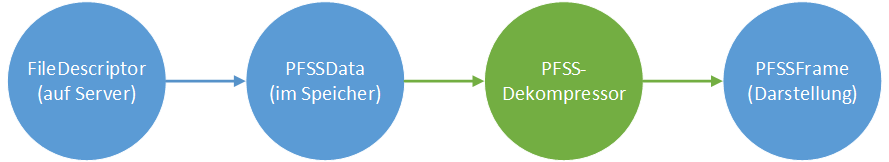
\includegraphics[width=0.8\textwidth,height=6cm,keepaspectratio]{./pictures/implementation/dataflow.png}
	\caption{Zustandsdiagramm der Feldliniendaten}
	\label{implementation:architektur:datenfluss}
\end{figure}
Die Daten der Feldlinien durchlaufen im JHelioviewer vier Zustände, welche durch vier Klassen abgebildet wurde. Die Klassen sowie die Zustandswechsel sind im Diagramm der Abbildung \ref{implementation:architektur:datenfluss} dargestellt. Die Klasse ''FileDescriptor´´ repräsentiert eine Aufnahme von Feldlinien auf dem Server. In diesem Zustand sind die Daten bereit für das Herunterladen. Die folgende Klasse ''PFSSData´´ symbolisiert Feldlinien, welche in den lokalen Arbeitsspeicher geladen wurden. In diesem Zustand sind die Daten noch komprimiert und nicht bereit für eine Visualisierung. Für das Herunterladen ist ebenfalls die ''PFSSData´´ Klasse zuständig. ''PFSSDekompressor´´ ist ein Zwischenzustand und stellt den Wechsel von komprimierten zu unkomprimierten Daten dar. Da der Zustandswechsel aufwändig ist, wird es durch eine eigene Klasse abgebildet. Die letzte Klasse ''PFSSFrame´´ repräsentiert die dekomprimierten Feldlinien. In diesem Zustand sind die Daten bereit für die Darstellung. Die Darstellung wird ebenfalls von der ''PFSSFrame´´ Klasse übernommen.

\subsubsection{Mehrstufiges Vorladen und Caching}
Um den Flaschenhals herunterladen und Dekomprimieren zu umgehen, wird ein mehrstufiges Read-Ahead und Caching eingeführt. Es soll ein Read Ahead und Caching für die unkomprimierten ''PFSSFrame´´ Feldllinien und eines für die ''PFSSData´´ Objekte implementiert werden. Für das wurde folgende Klassen implementiert:
(Klassendiagramm)
Der FileDescriptorManager
Die Klasse ''Framemanager´´ stellt die erste Stufe dar des Vorladens dar. Sie ist dafür zuständig, das aktuelle ''PFSSFrame´´ Objekt und eine bestimmte Anzahl von folgenden Aufnahmen im speicher zu behalten. Falls Aufnahmen fehlen, werden sie vom FrameCache anzufordern. Der Framemanager ist selbst für das Vorladen zuständig. Da die ''PFSSFrame´´ Objekte jeweils Speicher auf der Grafikkarte alloziieren und abräumen müssen, muss der Framemanager genau wissen, wann ein PFSSFrame Objekt neu geladen oder nicht mehr gebraucht wird. Die Klasse FrameCache nur noch zuständig, PFSSFrame Objekte zwischenzuspeichern, welche keine Ressourcen der Grafikkarte alloziiert haben. Es ist auch eine Architektur denkbar, inder der FrameCache das Vorladen und das Abräumen des Grafikkartenspeichers übernimmt. Der Speicherplatz der Grafikkarte würde aber die Grösse des FrameCaches beschränken.\\
Das Vorladen und Caching der PFSSData Objekten wird von der Klasse DataCache übernommen. Die PFSSData Objekte alloziieren nur Arbeitsspeicher, die vom Garbage-Collector aufgeräumt werden können. Das Vorladen ist deshalb simpler und wird direkt im DataCache implementiert durch eine weitere Instanz des LRUCaches. Der eigentliche Cache beinhaltet alle PFSSData Objekte, welche gebraucht wurden und der readAheadCache alle, welche noch gebraucht werden können.\\
[\baselineskip] 
Der JHelioviewer fragt im allgemeinen Fall sequenzell nach den Datenobjekten. Das bedeutet, dass ein LRU Cache sehr simpel mit einer First-in-First-out Queue implementiert werden kann. Das Objet, welches am längsten nicht mehr gebraucht wurde, ist das Letzte in der Queue.\\
Der LRU-Cache funktioniert gut, wenn die Anzahl Objekte deutlich grösser ist, als der Cache zu halten mag. Der LRU-Cache versagt aber beim Wrap-Around. Wenn es aber $n$ Objekte gibt und der Cache $n-1$ Objekte speichern kann, so löscht er immer das Nächste Objekt, welches gebraucht wird. 

\subsubsection{Asynchrone Aufrufe mittels Executor Services}
Um vom Preload und Caching sinnvoll gebrauch zu machen, muss die Dekompression und das Herunterladen der Feldlinien asynchron implementiert sein. Dazu müssen alle Klassen aus Abbildung \ref{implementation:architektur:datenfluss} threadsafe sein.
Die Klasse FileDescriptor ist einfach, diese ist Immutable und somit Threadsafe.
PFSSData und Frame threadsafe, data + compressor implementieren runnable
Nun Creators verwenden den Executor Service für bla


